\subsection{Method Overview}
\label{sec:method_overview}

The method iteratively estimates and refines a map point's existence probability \(\estpe\) through the integration of new observations \(\observation\) and historical, viewpoint-dependent observability priors. This is accomplished with an observability model and a Bayesian Existence Probability Estimator (EPE). The observability model provides \(\estpsge\), which \(\epe\) uses to update \(\estpe\) given each new \(\observation\). This chapter gives an overview of the full \vbee{} framework, followed by a detailed description of the observability modeling approach, the EPE, and how overall observability influences the update.

\subsubsection{The \vbee{} Framework}

The \vbee{} framework combines an observability model with the \epe. The high-level structure is shown in Figure \ref{fig:existence_estimation_framework}.

% TODO: Add feedback line
\begin{figure}[!ht]
    \centering
    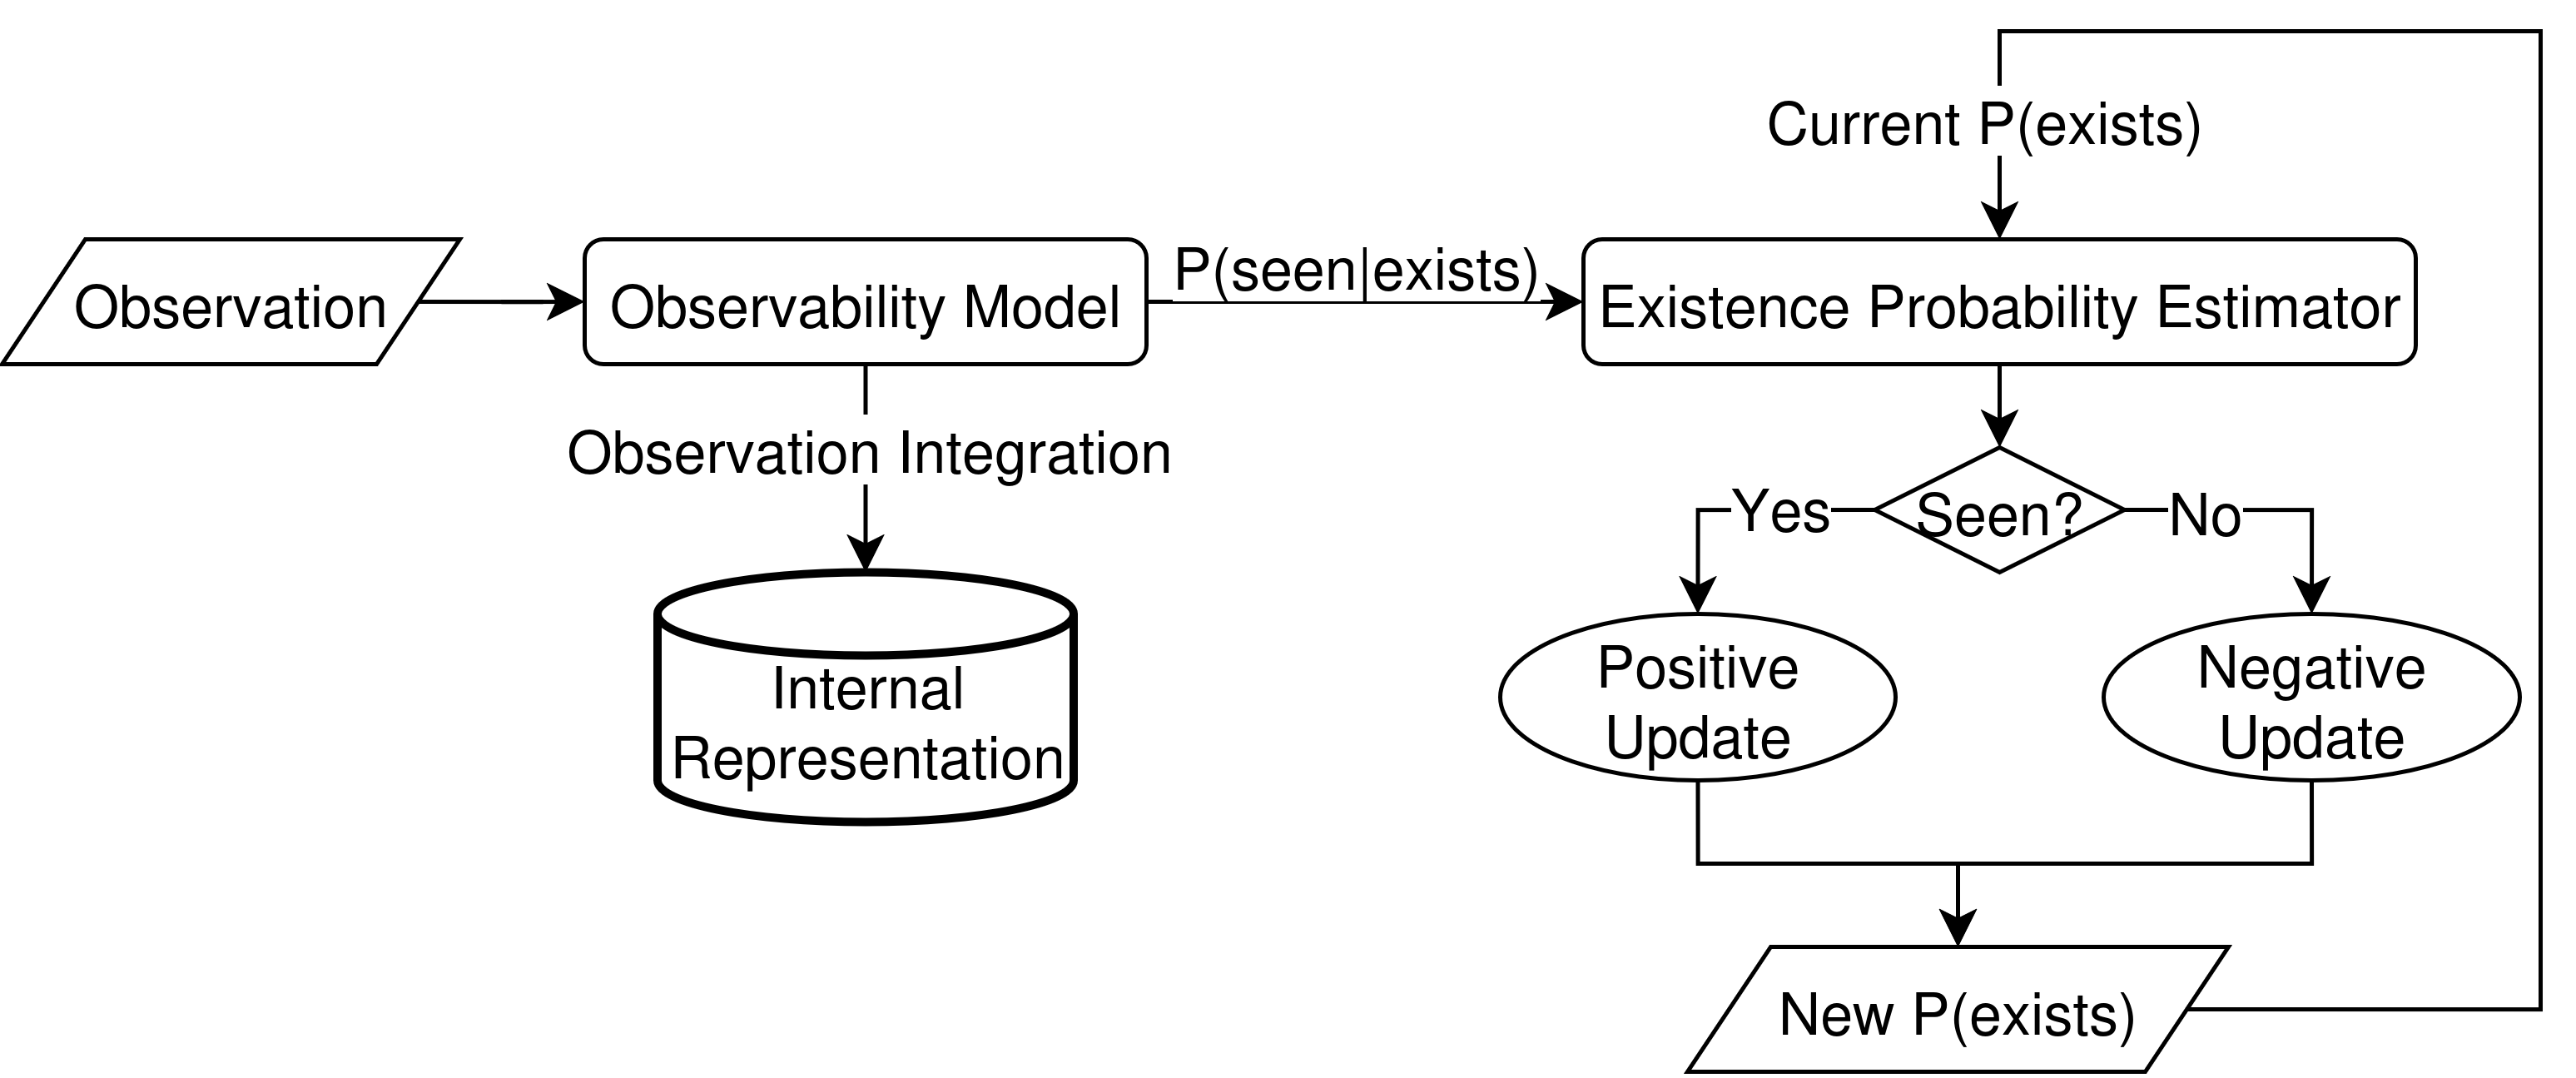
\includegraphics[width=0.7\textwidth]{resources/existence_estimation_framework.png}
    \caption[VBEE Framework]{A flowchart representing the flow of data through the proposed VBEE framework.}
    \label{fig:existence_estimation_framework}
\end{figure}

The observability model estimates \(\psge\), the probability of observing a map point from a given viewpoint \(\viewpoint\) (given the point exists), based on historical observations. That estimate \(\estpsge\) is consumed by the \epe, which updates \(\estpe\) using a Bayesian update. The new observation \(\observation\) is then integrated into the model via \(\integrate{\observation,\feedback}\), where feedback \(\feedback\) from the \epe\ (\(\feedback \!=\! \estpe_t - \estpe_{t-1}\)) modulates the impact of \(\observation\) on the model.

\subsubsection{The Observability Model}

Map points are conceptualized as static, infinitesimally small points in 3D Euclidean space. Let the observability of a map point \(p\) from a viewpoint \(\viewpoint \in \viewpointdomain\) be represented by
\[
    \operatorname{observable}_p : \viewpointdomain \to \{0,1\},
\]
where \(\viewpoint\) can be parameterized by azimuth, elevation, and distance (e.g., \(\{\theta,\phi,d\}\)). This function returns \(1\) if \(p\) is observed from \(\viewpoint\), and \(0\) otherwise. An observation is \(\observation=(\viewpoint,\state)\) and a set of \(n\) observations is \(\observations{n}=\{\observation_0,\dots,\observation_n\}\). For illustrative purposes, figures may use a simplified 2D representation \(\{\theta,d\}\). Figure \ref{fig:global_observability_p} shows such a plot representing the global observability of a map point \(p\) and the effects of obstructions.

\begin{figure}[!ht]
    \centering
    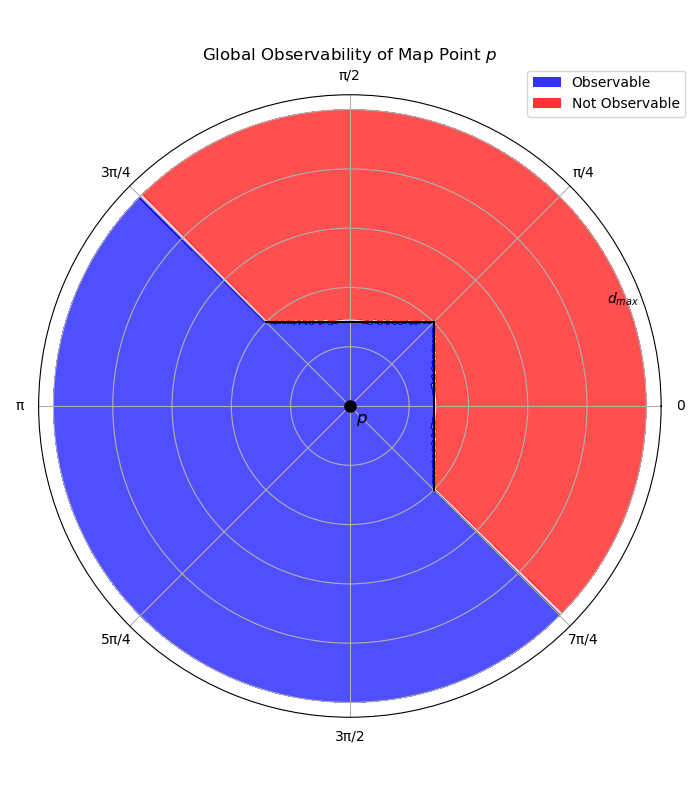
\includegraphics[width=0.7\textwidth]{resources/global_observability_p.png}
    \caption[2D Global Observability]{A 2D representation of the global observability of a map point \(p\) near two orthogonal obstructions.}
    \label{fig:global_observability_p}
\end{figure}

Generating such a plot exactly would require infinitely many observations across \(\viewpointdomain\). As stated in Section \ref{sec:objectives}, the model size should be small and effectively constant, so the model must operate on a fixed history and/or constant-size metadata.

The observability model exposes two functions: \(\estimate{\viewpoint}\), which returns \(\estpsge\), and \(\integrate{\observation,\feedback}\), which updates the internal representation. The goal is to minimize
\[
    \int_{\viewpointdomain} \big|\;\estimate{\viewpoint} \;-\; \operatorname{observable}_p(\viewpoint)\;\big| \, d\viewpoint,
\]
the total error between the model’s estimate and the true observability of \(p\).

\subsubsection{Existence Probability Estimator}

The \epe{} updates \(\estpe\) based on \(\observation\) and \(\estpsge\) using Bayes’ rule:
\[
    \estpe_{t+1} =
    \begin{cases}
        \displaystyle \frac{\psge\,\estpe_t}{P(S^{\viewpoint})} & \text{given } S^{\viewpoint}, \\[8pt]
        \displaystyle \frac{(1-\psge)\,\estpe_t}{P(\neg S^{\viewpoint})} & \text{given } \neg S^{\viewpoint},
    \end{cases}
\]
with marginals
\[
    P(S^{\viewpoint}) = \psge\,\estpe_t + \underbrace{P(S^{\viewpoint}\mid \lnot E)}_{\falsepos}\,(1-\estpe_t), \qquad
    P(\neg S^{\viewpoint}) = (1-\psge)\,\estpe_t + (1-\falsepos)\,(1-\estpe_t).
\]
Here, \(\falsepos \equiv P(S^{\viewpoint}\mid \lnot E)\) models the false-positive rate (e.g., spurious matches), to be set empirically in Section \ref{sec:existence_confidence_eval}. Substituting, the updates can be written compactly as
\[
    \estpe_{t+1} =
    \begin{cases}
        \displaystyle \frac{\psge\,\estpe_t}{\psge\,\estpe_t + \falsepos(1-\estpe_t)} & \text{given } S^{\viewpoint}, \\[10pt]
        \displaystyle \frac{(1-\psge)\,\estpe_t}{(1-\psge)\,\estpe_t + (1-\falsepos)(1-\estpe_t)} & \text{given } \neg S^{\viewpoint}.
    \end{cases}
\]

\subsubsection{Overall Observability}

If \(\estimate{\viewpoint}=1\) at some \(\viewpoint\), a single negative observation there could drive \(\estpe\) unrealistically low. To temper instantaneous updates, we apply a smoothing weight \(\damping \in [0,1]\):
\[
    \estpe_{t+1} \leftarrow (1-\damping)\,\estpe_t \;+\; \damping \cdot
    \begin{cases}
        \displaystyle \frac{\psge\,\estpe_t}{\psge\,\estpe_t + \falsepos(1-\estpe_t)} & \text{given } S^{\viewpoint}, \\[10pt]
        \displaystyle \frac{(1-\psge)\,\estpe_t}{(1-\psge)\,\estpe_t + (1-\falsepos)(1-\estpe_t)} & \text{given } \neg S^{\viewpoint}.
    \end{cases}
\]

Beyond instantaneous damping, we track an overall observability accumulator \(\observability\) that reflects the proportion of viewpoints from which the point tends to be observable. The accumulator is updated by comparing the Observation Status \(\state\in\{0,1\}\) to the model prediction \(\psge\):
\[
    \observability_{t+1} \;=\; (1-\damping)\,\observability_t \;+\; \observabilityupdate \,\big(\,\state \;-\; \psge\,\big).
\]
Intuitively, unexpected positive observations (\(\state=1\) when \(\psge\) is low) increase \(\observability\); unexpected negatives decrease it. The feedback signal \(\feedback=\estpe_{t+1}-\estpe_t\) is provided to \(\integrate{\observation,\feedback}\) so the observability model can adapt its internal state accordingly.
